\section{Modeling}\label{sec:modeling}
In order to model the Jao Gap we evolve two extremly finely sampled mass grid
of models. One of these grids uses the OPAL high-temperature opacity tables
while the other uses the OPLIB tables. Each grid evolves a model every 0.00025
$M_{\odot}$ from 0.2 to 0.4 $M_{\odot}$ and every 0.005 $M_{\odot}$ from 0.4 to
0.8 $M_{\odot}$. All models in both grids use a GS98 solar composition, the (1,
101, 0) \texttt{Free\_EOS} (version {\color{red}2.7}) configuration, and 1000
year old pre-main sequence polytropic models as their initial conditions.

Because in this work we are just interested in the location shift of the gap as
the opacity source varies, we do not model variations in composition.
{\color{red} Others have done this and they have found blah....}

The variability leading to the gap is quite clear in the mass luminosity
relation (Figures \ref{fig:OPALPunchIn} \& \ref{fig:OPLIBPunchIn}
{\color{red} Make this figure for the two large runs})

\begin{figure}
	\centering
	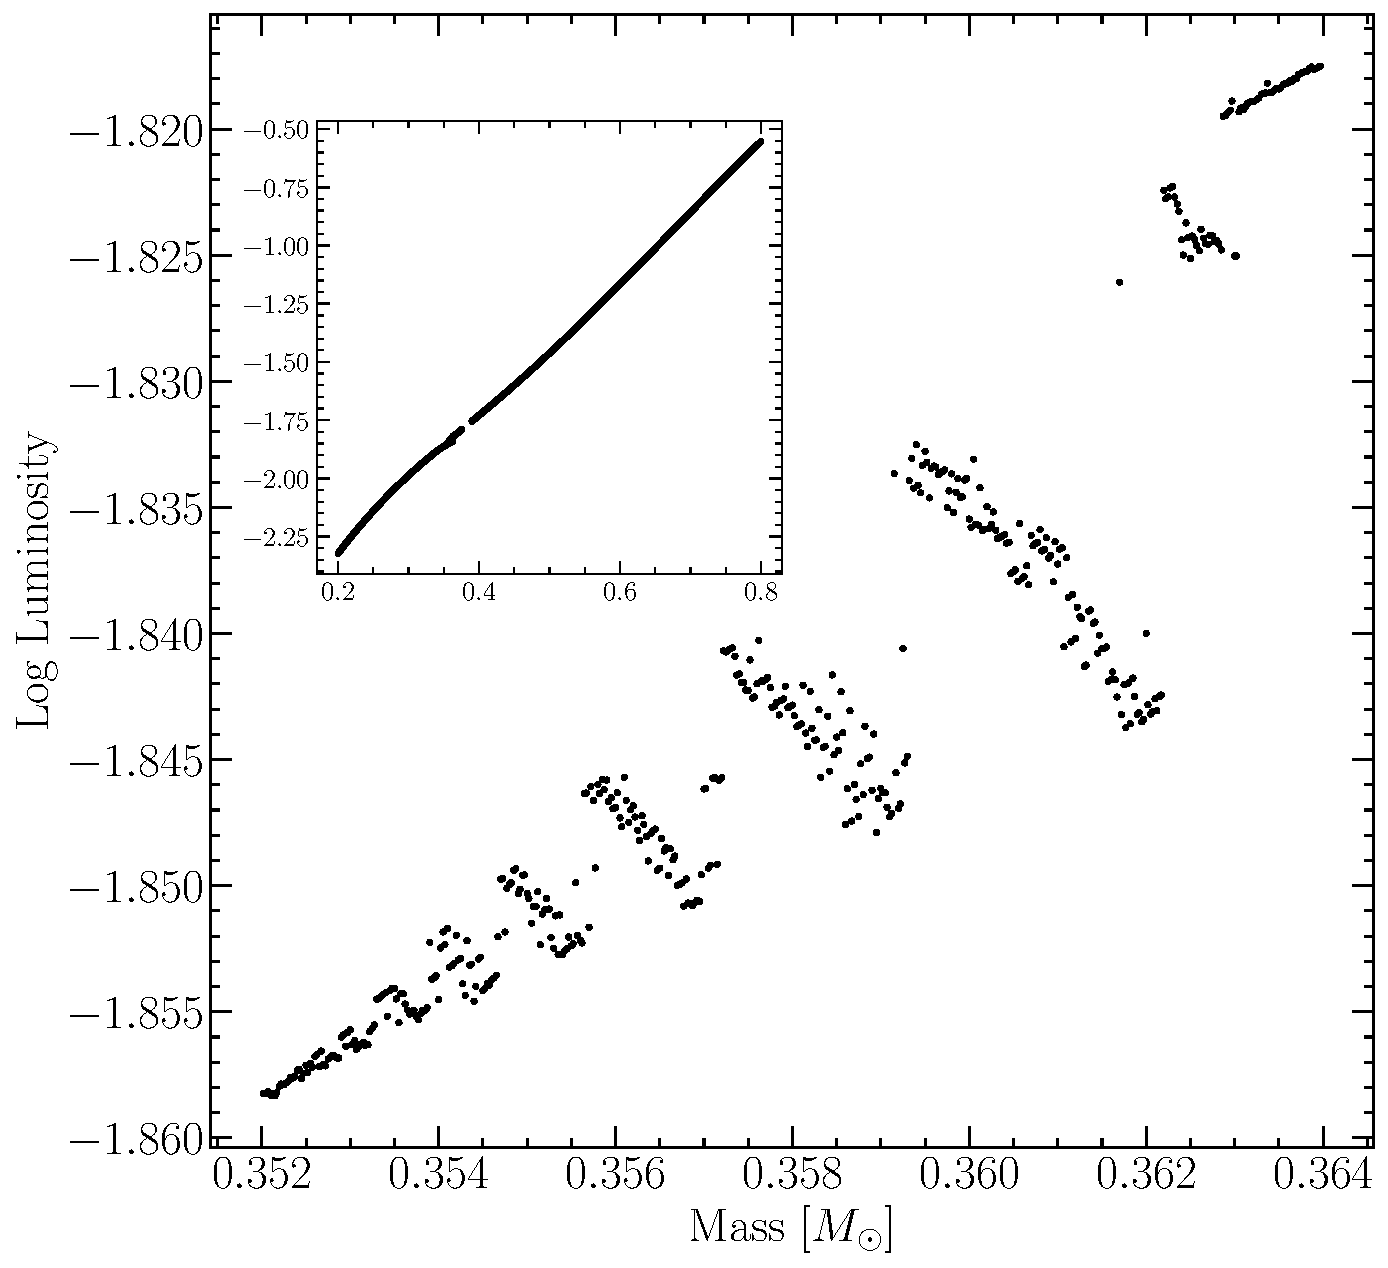
\includegraphics[width=0.45\textwidth]{src/figures/NotebookFigs/OPALPunchIn.pdf}
	\caption{{\color{red} THIS IS A TEST FIGURE, REPLACE WHEN LARGE RUN IS DONE}}
	\label{fig:OPALPunchIn}
	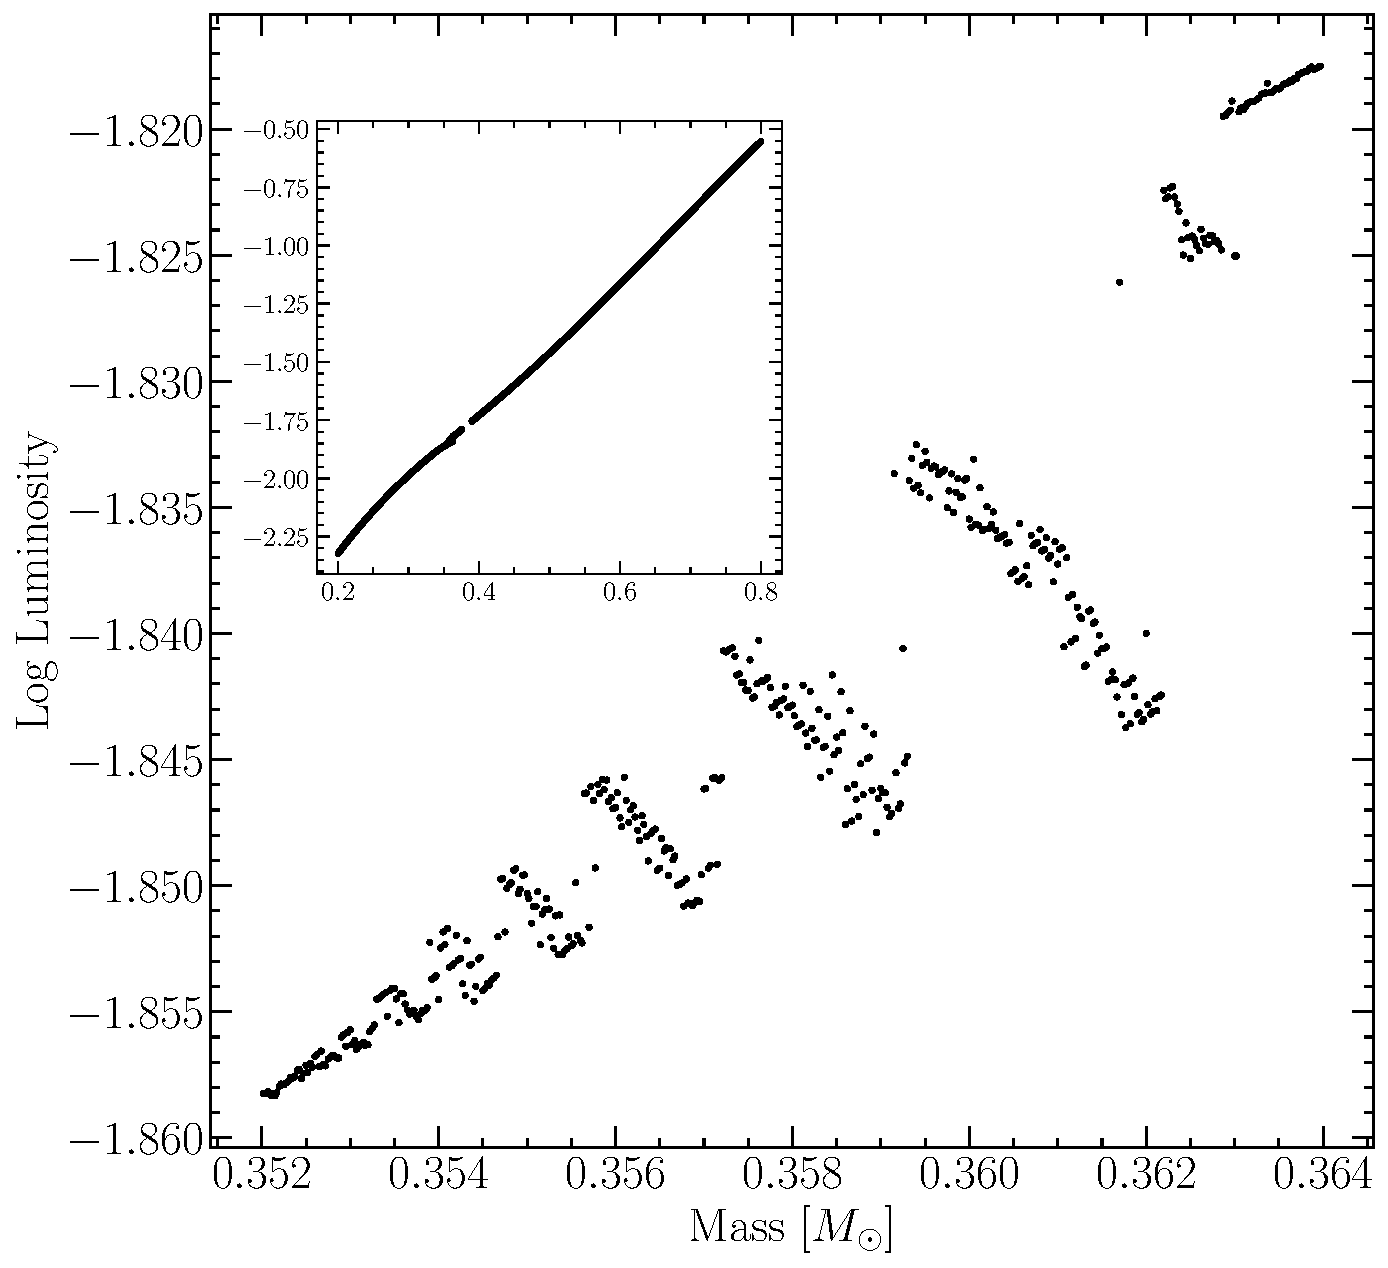
\includegraphics[width=0.45\textwidth]{src/figures/NotebookFigs/OPALPunchIn.pdf}
	\caption{{\color{red} THIS IS A TEST FIGURE, REPLACE WHEN LARGE RUN IS DONE}}
	\label{fig:OPLIBPunchIn}
		
\end{figure}

\subsection{Population Synthethis}
In order to compare the gap to observations we use in house population
synthetis code. Our population synthetis code first uses inverse CDF sampling
to build a distribution of target masses from some initial mass function (IMF).
Specifically we use the \citeauthor{Sollima2019} IMF where, for masses 0.25
$M_{\odot}$ < $M$ < 1 $M_{\odot}$, $\alpha=-1.34\pm0.07$. The model nearest in
mass to the samples mass above and the nearest model below are then selected
from the evolved database. The surface gravity, luminosity, and effective
temperature of the sample are then estimated through computing a linear
interpolation between the bounding models and evaluating that interpolation at
the sample mass. $T_{eff}$, $g$, and $log(L)$ are transformed into Gaia G, BP,
and RP magnitudes using the bolometric corrections provided by the Gaia
Colaboration, specifically \texttt{fehp000.UBVRIplus} {\color{red}[CITATION]}
{\color{red}[How to cite Aarons code]}. Next, we introduce observationally
informed photometric and astrometric Uncertainties into our population.

We select the Gaia Catalogue of Nearby Stars (GCNS) {\color{red}[CITATION]} to
empirically calibrate uncertainty relations. A function with the form of
Equation \ref{eqn:plxCalib} is fit to parallax uncertainty vs. G magnitude.
Additionally, a function of the form of Equation \ref{eqn:MagCalib} is fit to
to i$^{\text{th}}$ (G, BP, RP) magnitude uncertainty vs. i$^{\text{th}}$
magnitude.

\begin{align}\label{eqn:plxCalib}
	\sigma_{plx}(M_{g}) = ae^{bM_{g}}+c
\end{align}
\begin{align}\label{eqn:MagCalib}
	\sigma_{i}(M_{i}) = ae^{M_{i}-b}+c
\end{align}

Each of these functions then gives the an estimated uncertainty of some
quantity at a given magnitude. For each sampled star in the synthetic
population we select a parallax from the GCNS, refered to as the ''true
parallax''. This selection follows the distribution given in Figure
{\color{red} MAKE A FIGURE PLOTTING p from fromTagger.py in ThomasAstro on line
39 in that file}. A parallax uncertainty is calculated based on the G magnitude
magnitude of the synthetic star (hereafter the ``true G magnitude) and the
results of the fitting described in the previous paragraph. This uncertainty
then will, with equal weighting, either be added or subtracted from the true
parallax, yeilding an ``observed parallax''. The true parallax will be used to
convert the true i$^{\text{th}}$ magnitude to an apparent i$^{\text{th}}$
magnitude and the observed parallax will be used to convert the apparent
i$^{\text{th}}$ magnitude into an observed i$^{\text{th}}$ magnitude. Finally,
each observed magnitude is summed with an estimated uncertainty for that
magnitude based on the fit of the i$^{\text{th}}$ magnitude to the uncertainty
in the i$^{\text{th}}$ magnitude.

To summarize the process that each synthetic star will go through
\begin{enumerate}
	\item Sample from a \citet{Sollima2019} IMF to determine synthetic star mass
	\item Find the closest model above and below the synthetic star, linerally
		interpolate model parameters to the synthetic star mass.
	\item Convert synthetic star $g$, $T_{eff}$, and $Log(L)$ to Gaia G, BP,
		and RP colors.
	\item Sample from the GCNS to assign synthetic star a ``true'' parallax.
	\item Evaluate the empirical calibration given in Equation
		\ref{eqn:plxCalib} to find an associated parallax uncertainty and
		adjust the true parallax by this value resulting in an observed
		parallax.
	\item Use the true parallax to find an apparent magnitude for each filter.
	\item Use the observed parallax and the apparent magnitude to find an
		observed magnitude
	\item Evaluate the empirical calibration given in Equation
		\ref{eqn:MagCalib} to give a magnitude uncertainty scale in each band.
	\item Adjust each magnitude by some amount sampled from a normal
		distribution with a standard deviation of the magnitude uncertainty
		scale.
\end{enumerate}

This method then incorperats both photometric and astrometric Uncertainties
into our population synthetis. Seven Gyr old synthetic populations using OPAL
and OPLIB opacities are given in Figure \ref{fig:PopSynthCompareBasic}.

\begin{figure*}
	\centering
	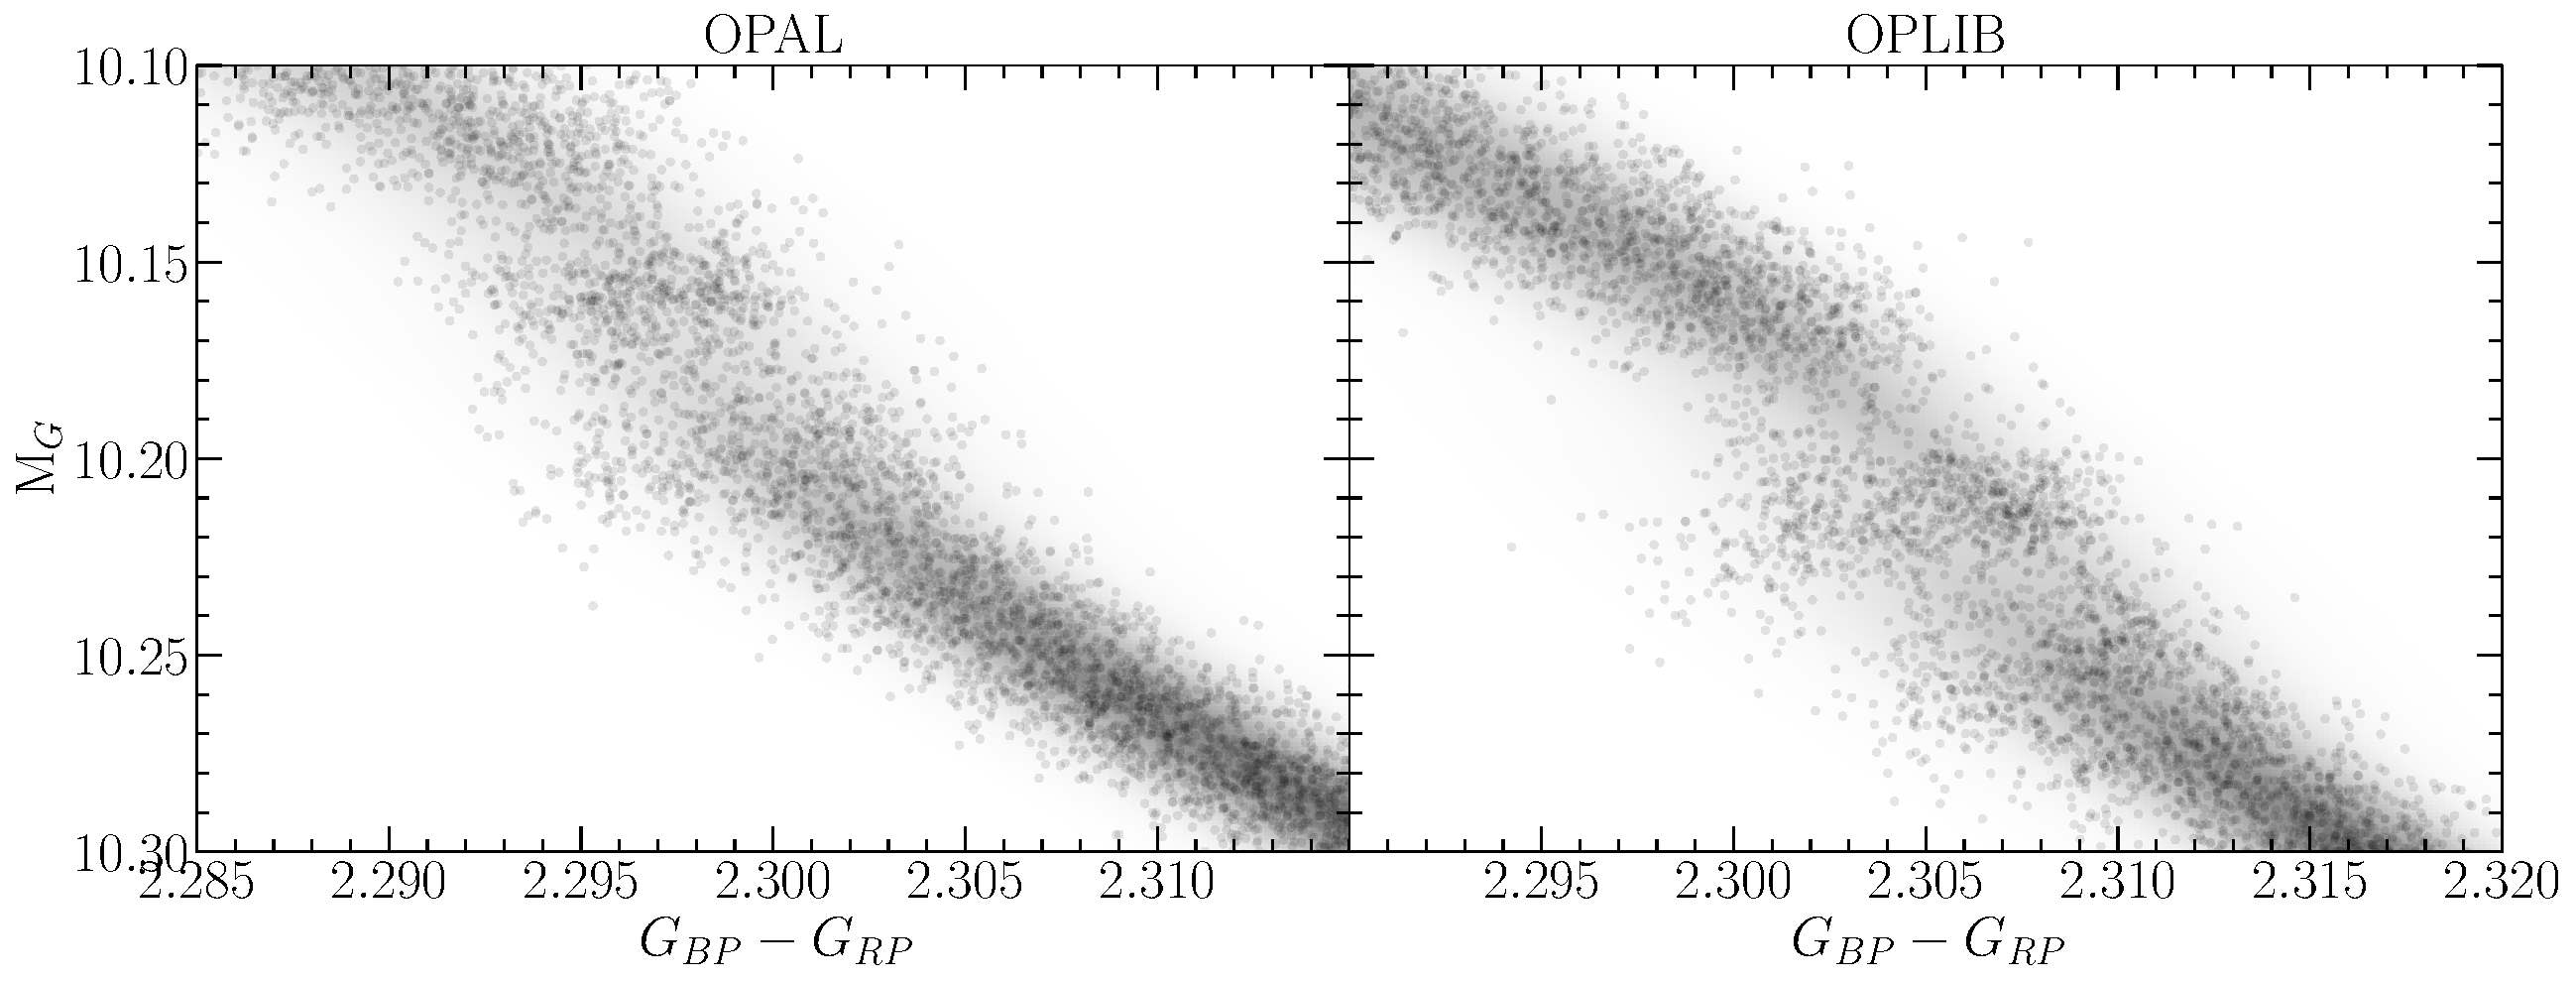
\includegraphics[width=0.85\textwidth]{src/figures/NotebookFigs/OPALOPLIB_popsynth_compare.pdf}
	\caption{Population synthetis resulst for models evolved with OPAL (left)
	and models evolved with OPLIB (right). A gaussian kernel-density-estimate
	has been overlayed to better highlight the density variations. {\color{red}
	[THIS IS A PLACEHOLDER FIGURE]}}
	\label{fig:PopSynthCompareBasic}
\end{figure*}
